\documentclass{beamer}
\usetheme{Frankfurt}
\usepackage{tikz}
\usepackage{booktabs}
\usepackage{graphicx}
\DeclareMathOperator{\id}{Id}
\newcommand{\fxpsi}{\Phi_{\theta}^{BA}}
\newcommand{\fxvarphi}{\Phi_{\theta}^{AB}}
\newcommand{\fxpsivarepsilon}{\Phi_{\theta \varepsilon}^{BA}}
\newcommand{\fxvarphivarepsilon}{\Phi_{\theta \varepsilon}^{AB}}
\graphicspath{{figs/}}

\title{Symmetries of the image registration problem}
\author{Hastings Greer}
\date{\today}


\begin{document}


\AtBeginSection[]
{
    \begin{frame}
        \frametitle{Table of Contents}
        \tableofcontents[currentsection,currentsubsection]
    \end{frame}
}
% Slide 1: Title
\begin{frame}
    \titlepage
\end{frame}

\section{Thesis and Notation}

\begin{frame}{Thesis Statement}
Image registration is a problem where the correct solution has inherent symmetries. By making this formal, and then restricting deep networks that solve the registration problem to have these same symmetries, we can regularize, simplify, and accelerate training while boosting performance.
\end{frame}

% Slide 2: Two-column text
\begin{frame}{Notation}
    \begin{columns}
        \column{0.6\textwidth}
	    $$I^A: \mathbb{R}^N \rightarrow \mathbb{R} $$

$$\Phi:
	\left( (\Omega \rightarrow \mathbb{R}) \times (\Omega \rightarrow \mathbb{R})
	\right) \rightarrow (\Omega \rightarrow \Omega) $$
        \column{0.4\textwidth}
	Basic loss:
	    $$ \mathcal{L}_{sim}(I^A \circ \Phi[I^A, I^B], I^B) i$$
	    $$+ \mathcal{L}_{reg}(\Phi)$$

	    Note that $\mathcal{L}_{reg}$ is operating on $\Phi$ and so can, e.g., call it with various arguments
    \end{columns}
\end{frame}

% Slide 2: Two-column text
\begin{frame}{The important symmetries}
    \begin{columns}
        \column{0.4\textwidth}
Inverse Consistency 
\vskip 1em
            $\Phi[I^A, I^B] \circ \Phi[I^B, I^A] = Id$
        \column{0.6\textwidth}
Equivariance
\vskip 1em
            $\Phi[W \circ I^A, U \circ I^B] = W^{-1} \circ \Phi[I^A, I^B] \circ U$
    \end{columns}
\end{frame}


\section{ICON}
\begin{frame}{Regularizing a real registartion problem via Inverse Consistency}
	\begin{columns}
		\column{.5\textwidth}
        \begin{itemize}
            \item Dataset: OAI Knees, ~40,000 MRI Images
		   \item Neural Network Architecture: Stacked U-Nets, 2 step half res, 2 step full res
		   \item ADAM Optimization
		   \item Loss function: $\mathcal{L} = [I^A \circ \Phi[I^A, I^B], I^B]]^2_2 + \lambda [\Phi[I^A, I^B] \circ \Phi[I^B, I^A] - Id ]^2_2$
        \end{itemize}
		\column{.5\textwidth}
		\includegraphics[width=1\textwidth]{orals/Screenshot 2024-08-30 at 2.29.56 AM.png}
	\end{columns}
\end{frame}

\begin{frame}{The Leaderboard}
	\includegraphics[width=1\textwidth]{orals/Screenshot 2024-08-30 at 2.35.06 AM.png}
\end{frame}

\begin{frame}{What is a diffeomorphism?}
	\begin{columns}
		\column{.5\textwidth}
	\begin{itemize}
		\item Any function $\mathcal{R}^N \rightarrow \mathcal{R}^N $with two properties:
		\item Differentiable
		\item Has differentiable inverse
		\item i.e. no folds
		\item We desire $\Phi[I^A, I^B]$ diffeomorphic

	\end{itemize}
	
		\column{.5\textwidth}

		\includegraphics[width=1\textwidth]{orals/Screenshot 2024-08-30 at 2.39.46 AM.png}
	\end{columns}
\end{frame}

\begin{frame}{A vision of simpler registration}
	\begin{itemize}
		\item if $\Phi[I^A, I^B]$ is represented as piecewise linear, it is differentiable (close enough)
		\item if $\Phi[I^A, I^B] \circ \Phi[I^B, I^A] = Id$, then $\Phi[I^A, I^B]$ is invertible
		\item Done!
	\end{itemize}
\end{frame}

\begin{frame}{Why smooth? two hypotheses}
	\begin{columns}
		\column{.5\textwidth}
	\begin{itemize} 
		\item Perhaps we are getting smoothing from the dataset?
		\item Perhaps we are getting smoothing from Inverse Consistency alone?
	\end{itemize}
		\column{.5\textwidth}
		\includegraphics[width=1\textwidth]{orals/Screenshot 2024-08-30 at 2.29.56 AM.png}
	\end{columns}
	\end{frame}
\begin{frame}{Is it the dataset?}
	\begin{columns}
		\column{.5\textwidth}
	\begin{itemize} 
		\item Dataset: Single pair of images
		\item Neural network: MLP
		\item $\Phi[](x) = x + interpolate(MLP(I^A, I^B), x)$
		   \item Loss function: $\mathcal{L} = [I^A \circ \Phi[I^A, I^B], I^B]]^2_2 + \lambda [\Phi[I^A, I^B] \circ \Phi[I^B, I^A] - Id ]^2_2$
	\end{itemize}
		\column{.5\textwidth}
		\includegraphics[width=1\textwidth]{orals/Screenshot 2024-08-30 at 2.59.26 AM.png}
	\end{columns}
	\end{frame}
\begin{frame}{Is it the loss alone?}
	\begin{columns}
		\column{.5\textwidth}
	\begin{itemize} 
		\item Dataset: Single pair of images
		\item $G^{AB}, G^{BA}$ Grids of vectors initialized to zero
		\item $\Phi[](x) = x + interpolate(G^{AB}, x)$
		   \item Loss function: $\mathcal{L} = [I^A \circ \Phi[I^A, I^B], I^B]]^2_2 + \lambda [\Phi[I^A, I^B] \circ \Phi[I^B, I^A] - Id ]^2_2$
	\end{itemize}
		\column{.5\textwidth}
		\includegraphics[width=1\textwidth]{orals/Screenshot 2024-08-30 at 3.01.59 AM.png}
	\end{columns}
	\end{frame}

	\begin{frame}{So, What's the Difference?}
		\begin{itemize}
			\item Mystery: network on single pair works, grid on single pair doesn't work
			\item: A clue: maps with small jacobian amplify error
		\end{itemize}
		\includegraphics[width=1\textwidth]{orals/Screenshot 2024-08-30 at 3.06.04 AM.png}
	\end{frame}
\begin{frame}{Implicit Regularization}

{\centering
\scalebox{0.90}{\parbox{1.12\linewidth}{%
\begin{equation}
\begin{split}
 \mathcal{L}_{\text{inv}} & \approx \left\| \fxvarphi \circ \fxpsi - \operatorname{Id}\right\|^2_2  + \left\| \fxpsi \circ \fxvarphi - \operatorname{Id}\right\|^2_2 \\
  + \varepsilon^2 &\left\| \mathrm{d} \fxvarphi \sqrt{\operatorname{Jac}(\fxvarphi)} \right\|^2_2 
  + \, \varepsilon^2 \left\| \mathrm{d} \fxpsi \sqrt{\operatorname{Jac}(\fxpsi)} \right\|^2_2\, .
  \end{split}
  \label{EqH1regularization}
\end{equation}
}}}
\end{frame}

\begin{frame}{New Hypothesis}
	The reason that the 2-data-point neural network is regularized while the grid of vectors isn't, is that the neural network is noisy

	If we add some gaussian noise to the grid of vectors, does it become regularized?
\end{frame}

\begin{frame}{Noise regularizes the grid-of-vectors-ICON}
	\begin{columns}
		\column{.5\textwidth}
	\begin{itemize} 
		\item Dataset: Single pair of images
		\item $G^{AB}, G^{BA}$ Grids of vectors initialized to zero
		\item $\Phi[](x) = x + interpolate(G^{AB} + \mathcal{N}(\epsilon), x)$
		   \item Loss function: $\mathcal{L} = [I^A \circ \Phi[I^A, I^B], I^B]]^2_2 + \lambda [\Phi[I^A, I^B] \circ \Phi[I^B, I^A] - Id ]^2_2$
	\end{itemize}
		\column{.5\textwidth}
		\includegraphics[width=1\textwidth]{orals/Screenshot 2024-08-30 at 7.11.28 AM.png}
	\end{columns}
	\end{frame}

	\begin{frame}{ICON: impractical at high resolution}
		\includegraphics[width=1\textwidth]{orals/Screenshot 2024-08-30 at 7.16.19 AM.png}
	\end{frame}

\section{GradICON}

\begin{frame}{Need resolution invariant version of ICON loss}
	\begin{columns}
		\column{.5\textwidth}
	\begin{itemize}
		\item Where to look?
		\item a non-invertible pixel requires a displacement that scales as voxel stride, 
		\item but a gradient that is invariant to voxel stride
		\item Try it, empirically the spatial gradient of the ICON loss works amazingly
	\end{itemize}
		\column{.5\textwidth}
		\includegraphics[width=1\textwidth]{orals/Screenshot 2024-08-30 at 7.51.14 AM.png}
	\end{columns}
	\end{frame}
\begin{frame}{GradICON}
	\begin{columns}
		\column{.5\textwidth}
	\begin{itemize}
		\item Loss function: $\mathcal{L} = \texttt{LNCC}[I^A \circ \Phi[I^A, I^B], I^B]]^2_2 + \lambda [\nabla[\Phi[I^A, I^B] \circ \Phi[I^B, I^A] - Id] ]^2_2$
		\item Difference: LNCC instead of SSD
		\item Difference: $\nabla$ in regularizer
	\end{itemize}
		\column{.5\textwidth}
		\includegraphics[width=1\textwidth]{orals/Screenshot 2024-08-30 at 7.51.14 AM.png}
	\end{columns}
	\end{frame}

	\begin{frame}{Engineering work: get to high performance on DirLab}
		\includegraphics[width=1\textwidth]{orals/Screenshot 2024-08-30 at 8.09.47 AM.png}
	\end{frame}

	\begin{frame}{Hurrah! hyperparameters tuned for DirLab generalize to other datasets}
	\begin{columns}
		\column{.5\textwidth}
		\includegraphics[width=.7\textwidth]{orals/Screenshot 2024-08-30 at 8.11.58 AM.png}
		\column{.5\textwidth}
		\includegraphics[width=1\textwidth]{orals/Screenshot 2024-08-30 at 8.12.29 AM.png}
	\end{columns}
	\end{frame}

\section{ConstrICON}

\begin{frame}
\vspace*{-1pt}
\makebox[\linewidth]{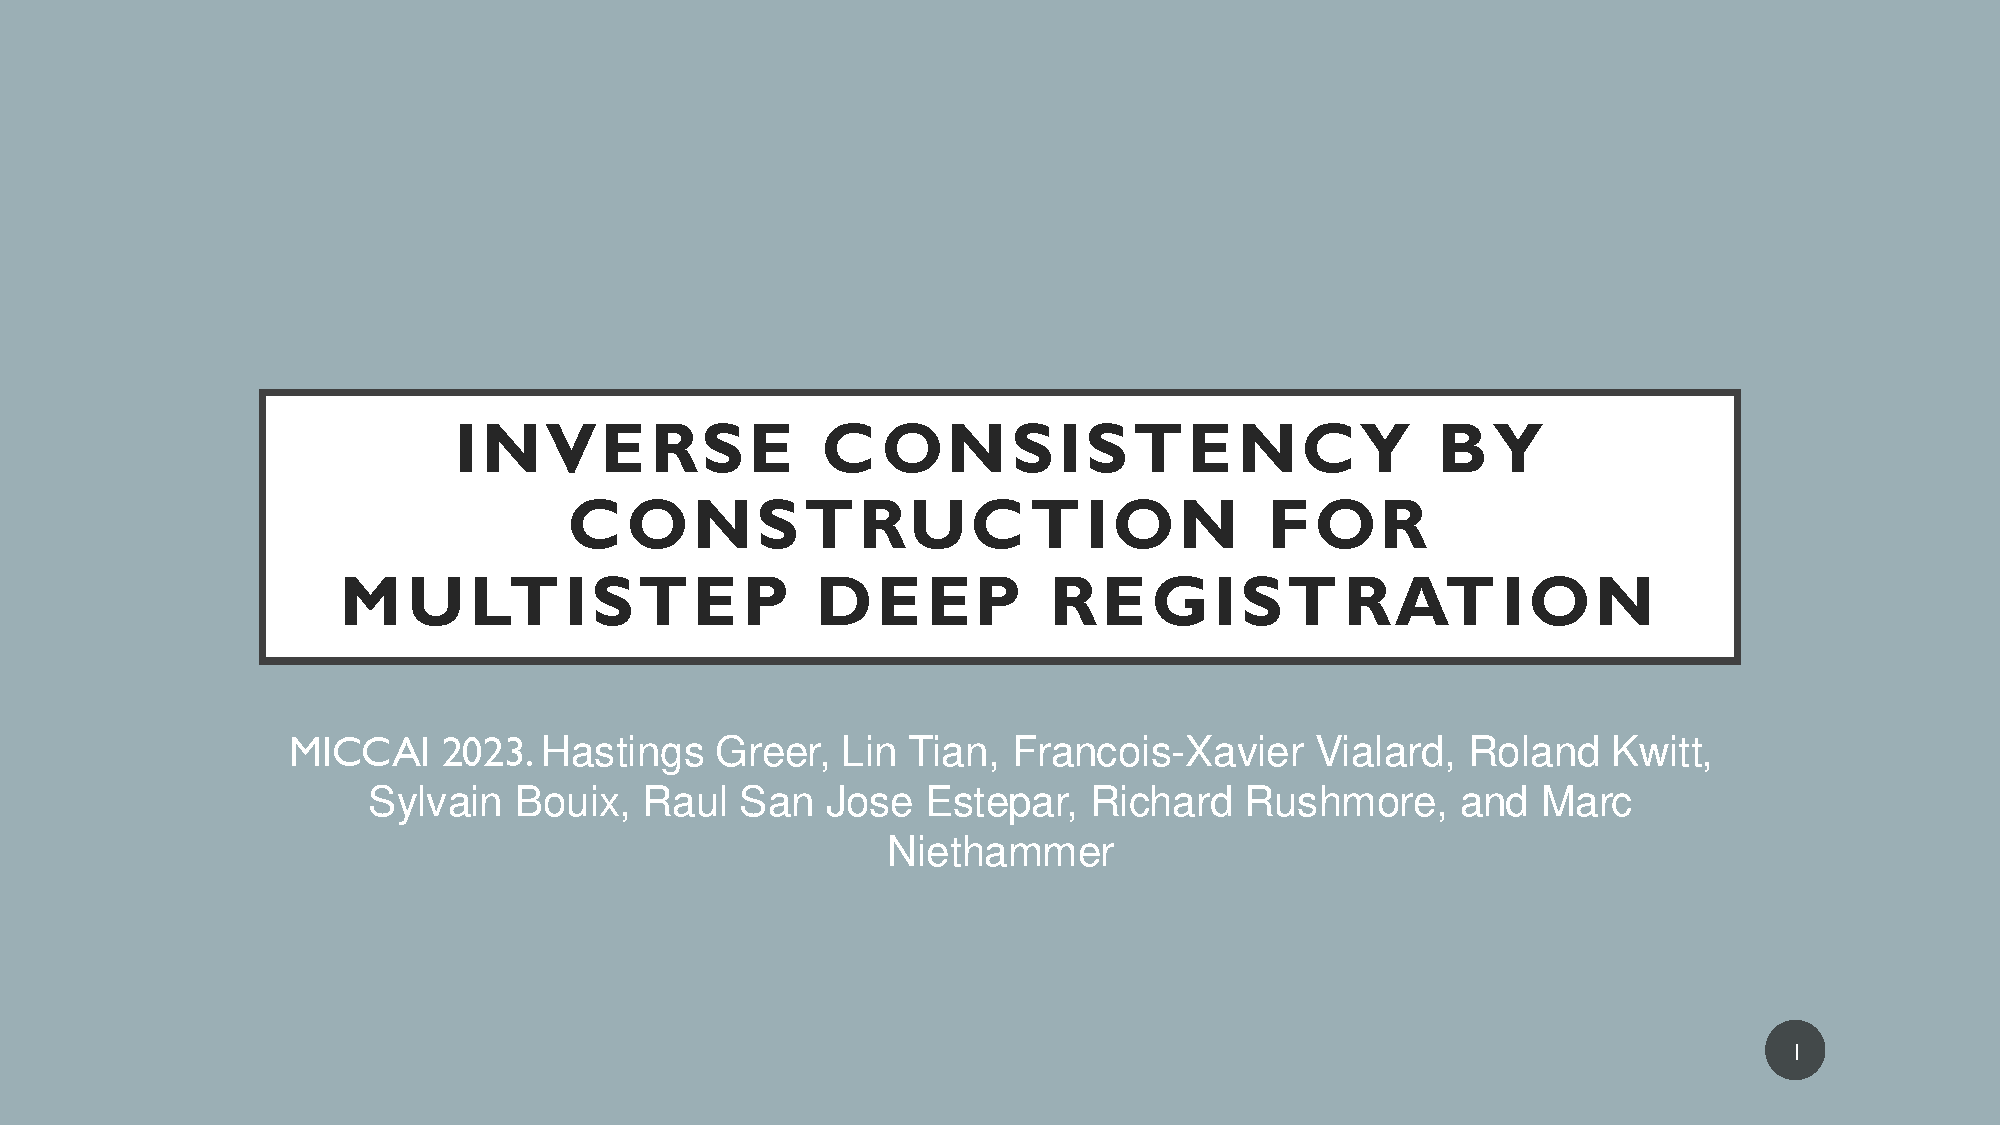
\includegraphics[page=1,width=\paperwidth]{ConstrICON presentation - miccai Talk - Narrative.pdf}}
\end{frame}

\begin{frame}
\vspace*{-1pt}
\makebox[\linewidth]{\includegraphics[page=2,width=\paperwidth]{ConstrICON presentation - miccai Talk - Narrative.pdf}}
\end{frame}
\begin{frame}
\vspace*{-1pt}
\makebox[\linewidth]{\includegraphics[page=3,width=\paperwidth]{ConstrICON presentation - miccai Talk - Narrative.pdf}}
\end{frame}
\begin{frame}
\vspace*{-1pt}
\makebox[\linewidth]{\includegraphics[page=4,width=\paperwidth]{ConstrICON presentation - miccai Talk - Narrative.pdf}}
\end{frame}
\begin{frame}
\vspace*{-1pt}
\makebox[\linewidth]{\includegraphics[page=5,width=\paperwidth]{ConstrICON presentation - miccai Talk - Narrative.pdf}}
\end{frame}
\begin{frame}
\vspace*{-1pt}
\makebox[\linewidth]{\includegraphics[page=6,width=\paperwidth]{ConstrICON presentation - miccai Talk - Narrative.pdf}}
\end{frame}
\begin{frame}
\vspace*{-1pt}
\makebox[\linewidth]{\includegraphics[page=7,width=\paperwidth]{ConstrICON presentation - miccai Talk - Narrative.pdf}}
\end{frame}
\begin{frame}
\vspace*{-1pt}
\makebox[\linewidth]{\includegraphics[page=8,width=\paperwidth]{ConstrICON presentation - miccai Talk - Narrative.pdf}}
\end{frame}
\begin{frame}
\vspace*{-1pt}
\makebox[\linewidth]{\includegraphics[page=9,width=\paperwidth]{ConstrICON presentation - miccai Talk - Narrative.pdf}}
\end{frame}
\section{Remaining Work}
\begin{frame}{Timeline}
	\begin{itemize} 
		\item October 9th:  Atlas + remove affine component submission to ISBI
		\item November: CARL resubmission to CVPR
		\item March: HugeGradICON submission to MICCAI
		\item May: Thesis defense
	\end{itemize}
\end{frame}
	
\section{CARL}

\begin{frame}{Coordinate Attention with Refinement Layers}
	Submitted to Neurips 2024, 4447.
	Waiting to hear back- will resubmit to CVPR if rejected
\end{frame}

\begin{frame}
\makebox[\linewidth]{
\includegraphics[page=2,width=\paperwidth]{Equivariant Image Registration-2.pdf}}
\end{frame}

\begin{frame}
\makebox[\linewidth]{
\includegraphics[page=3,width=\paperwidth]{Equivariant Image Registration-2.pdf}}
\end{frame}
\begin{frame}
\makebox[\linewidth]{
\includegraphics[page=4,width=\paperwidth]{Equivariant Image Registration-2.pdf}}
\end{frame}

\begin{frame}
\makebox[\linewidth]{
\includegraphics[page=5,width=\paperwidth]{Equivariant Image Registration-2.pdf}}
\end{frame}
\begin{frame}
\makebox[\linewidth]{
\includegraphics[page=6,width=\paperwidth]{Equivariant Image Registration-2.pdf}}
\end{frame}

\begin{frame}
\makebox[\linewidth]{
\includegraphics[page=7,width=\paperwidth]{Equivariant Image Registration-2.pdf}}
\end{frame}
\begin{frame}
\makebox[\linewidth]{
\includegraphics[page=8,width=\paperwidth]{Equivariant Image Registration-2.pdf}}
\end{frame}

\begin{frame}
\makebox[\linewidth]{
\includegraphics[page=9,width=\paperwidth]{Equivariant Image Registration-2.pdf}}
\end{frame}
\begin{frame}
\makebox[\linewidth]{
\includegraphics[page=10,width=\paperwidth]{Equivariant Image Registration-2.pdf}}
\end{frame}
\begin{frame}
\makebox[\linewidth]{
\includegraphics[page=11,width=\paperwidth]{Equivariant Image Registration-2.pdf}}
\end{frame}

\begin{frame}
\makebox[\linewidth]{
\includegraphics[page=12,width=\paperwidth]{Equivariant Image Registration-2.pdf}}
\end{frame}
\begin{frame}
\makebox[\linewidth]{
\includegraphics[page=13,width=\paperwidth]{Equivariant Image Registration-2.pdf}}
\end{frame}

\begin{frame}
\makebox[\linewidth]{
\includegraphics[page=14,width=\paperwidth]{Equivariant Image Registration-2.pdf}}
\end{frame}
\begin{frame}
\makebox[\linewidth]{
\includegraphics[page=15,width=\paperwidth]{Equivariant Image Registration-2.pdf}}
\end{frame}

\begin{frame}
\makebox[\linewidth]{
\includegraphics[page=16,width=\paperwidth]{Equivariant Image Registration-2.pdf}}
\end{frame}
\begin{frame}
\makebox[\linewidth]{
\includegraphics[page=17,width=\paperwidth]{Equivariant Image Registration-2.pdf}}
\end{frame}
\begin{frame}
\makebox[\linewidth]{
\includegraphics[page=18,width=\paperwidth]{Equivariant Image Registration-2.pdf}}
\end{frame}
\begin{frame}
	\includegraphics[width=1\textwidth]{orals/Screenshot 2024-08-30 at 9.46.53 AM.png}
\end{frame}
\section{Atlas Development}
\begin{frame}{Atlas Development}
	Marc needs registration of knees to 3-D atlas post-haste before UKBiobank access expires.

	Registration must have affine and deformable components seperated.

	Either equivariance by swapping out coordinate attention for KeyMorph or equivariance by instance optimizing an affine pre-registration achieves this.

	Atlas building code for mouse brains and diffusion images has been kicking around for a while, needs a home in a publication
\end{frame}

\begin{frame}{Atlas Development}
	\includegraphics[width=1\textwidth]{orals/Screenshot 2024-08-30 at 9.29.29 AM.png}
\end{frame}
\begin{frame}{Atlas Development}
	\begin{itemize}
		\item Plan: Score atlas creation and registration by DICE on knee through atlas and invariance of deformation field features to rigid [W, U] transforms.
		\item Submit 4 page paper to ISBI
		\item Submit deformation field features to local colaborator.
	\end{itemize}
\end{frame}

\section{HugeGradICON}
 \begin{frame}{HugeGradICON}
	 \begin{itemize}
		 \item uniGradICON and multiGradICON are registration foundation models built by our group from the GradICON architecture
		 \item Scaling dataset diversity and model size
		\item Practical focus: boost performance on real-world cases
		\item Unique insight from GitHub issues
	\end{itemize}
\end{frame}

\begin{frame}{Addressing Real-World Challenges}
	\begin{itemize}
		\item Non-brain-extracted images:
		\begin{itemize}
			\item Enforce brain extraction or improve performance without it
			\item Augment training set
			\item Potentially add open-source brain extraction to CLI
		\end{itemize}
		\item Handle images with black bars from resampling
		\begin{itemize}
		\item Label image / input image distinction strategy
			\item Augment training set
			\item potentially add cropping to CLI
		\end{itemize}
	\end{itemize}
\end{frame}

\begin{frame}{Multimodal Registration}
	\begin{itemize}
		\item Necessary for various applications
		\item Current findings:
		\begin{itemize}
			\item Improves multimodal task performance
			\item Harms unimodal task performance
		\end{itemize}
		\item Proposed solutions:
		\begin{itemize}
			\item Increase network capacity
			\item Add segentations via totalSegmentor
			\item Add SynthMorph shapes and brains datasets
		\end{itemize}
	\end{itemize}
\end{frame}

\begin{frame}{Additional Improvements}
	\begin{itemize}
		\item Explore rotational equivariance and exact inverse consistency
		\begin{itemize}
			\item ConstrICON
			\item CARL
		\end{itemize}
		\item Performance evaluation:
		\begin{itemize}
			\item Use tasks from GradICON, uniGradICON, and multiGradICON
			\item Allow easy comparison to current state-of-the-art
		\end{itemize}
	\end{itemize}
\end{frame}

\begin{frame}{Timeline and Submission}
	\begin{itemize}
		\item Focus after November CARL paper resubmission
		\item Target: MICCAI submission in March 2025
		\item Aim: Practical improvements for real-world usage
	\end{itemize}
\end{frame}



\begin{frame}{PhD Courses Overview}
    \begin{table}
        \scriptsize
        \begin{tabular}{llll}
            \textbf{Category} & \textbf{Course Number \& Title} & \textbf{Semester/Year} \\
            \hline
            A & Comp 790, Large Language Models & Fall 2022 \\
            T & Comp 782 Motion Planning & Spring 2021 \\
            T & Comp 755 Machine Learning & Fall 2020 \\
            A & Comp 790 Video Learning & Fall 2021 \\
            S & Comp 520 & Fall 2024 \\
            O & Math 680 Geometry of Curves and Surfaces & Fall 2020 \\
            \hline
            \multicolumn{3}{c}{\textbf{Additional Courses}} \\
            \hline
             & Math 750 Partial Differential Equations & Fall 2014 \\
             & Math 662 Scientific Computation II & Spring 2017 \\
             & Comp 776 Computer Vision of our 3D world & Spring 2021 \\
             & Math 668 Applied Math 1 & Fall 2022 \\
        \end{tabular}
    \end{table}

    \vspace{0.2cm}
    \tiny{
    Category Legend: A: Applications, T: Theory \& Formal Thinking,\\
    S: Systems \& Hardware, O: Outside of CS
    }
\end{frame}

\begin{frame}{Remaining Coursework}
        \begin{itemize}
            \item Operating Systems 630 Spring 2025
            \item Writing Spring 2025
        \end{itemize}
\end{frame}

\section{Oral examination}

\begin{frame}{Diffeomorphic Demons}
	\begin{itemize}
		\item Diffeomorphic Demons is a representative classical image registration approach.
		\item To preserve diffeomorphism: Store the transfrom as an element of the lie group, derive update in lie algebra, exponentiate and compose.
		\item Alternate minimizing least squares similarity and regularity. Least squares similarity update done using local linearization of similarity measure + constraint on step size.
		\item regularization can be done either by regularizing the algebra representation of the update (fluid-like) or regularizing the transform (diffusion-like). Authors prefer diffusion-like.

	\end{itemize}
\end{frame}

\begin{frame}{ANTs (Symmetric Normalization)}
	\begin{itemize}
		\item Wildly influential work on inverse consistent registration
		\item Algorithm: find a transform in two parts that brings the images to a common middle space
		\item Influence comes from performance + excellent software development: packaged along with affine pre-registration and great documentation of CLI and python wrapping

	\end{itemize}
\end{frame}
\begin{frame}{ConvexAdam}
	\begin{itemize}
		\item Compue ad-hoc per-pixel features
		\item Move each pixel in moving image to most similar pixel in fixed image
		\item Alternate: smooth displacement field, move each pixel to most similar pixel with penalty for distance from previous iteration.
		\item Convert to B-Spline, do local optimization with ADAM
		\item Key insight: first steps are tractable if SSD feature similarity is used, because convex
	\end{itemize}
\end{frame}

\begin{frame}{Voxelmorph}
        \begin{itemize}
              \item This paper lays out a simple approach to unsupervised neural registration
		\item $ \Phi_\theta[I^A, I^B](\vec{x}) := \text{Conv}_\theta[\text{cat}(I^A, I^B)](\vec{x}) + \vec{x} $
		\item minimize over a dataset $\mathcal{L} = \mathcal{L}_\text{sim}(I^A \circ \Phi_\theta[I^A, I^B], I^B] + \mathcal{L}_{reg}(\Phi_\theta[I^A, I^B])$
              \item It serves as a standard work for building on and comparing to

        \end{itemize}
\end{frame}

\begin{frame}{Probabilistic Voxelmorph}
        \begin{itemize}
              \item Two insights: First, pull from traditional registration to make diffeomorphic by construction:
	      \item $ \Phi_\theta[I^A, I^B](\vec{x}) := exp(\text{Conv}_\theta[\text{cat}(I^A, I^B)](\vec{x}))$
              \item Second, use a formulation similar to a variational autoencoder to formulate registration as finding the most likely transform

	      \item $  p(\text{fixed image} | \text{transform latent}; \text{moving image} ) = \mathcal{N}(\text{fixed image}; \text{moving image} \circ \phi_{\text{transform latent}}, \sigma^2)$

	      \item Then, transform regularity is just a gaussian prior on the transform latent

        \end{itemize}
\end{frame}
\begin{frame}{LapIRN (Laplacian Pyramid Image Registration Network)}
\begin{itemize}
\item Addresses challenges in deformable image registration for large displacements
\item Uses a Laplacian pyramid architecture for multi-scale registration
\item Key idea: Estimate displacement fields at multiple resolutions and progressively refine
\item Formula: $\phi = \phi_0 + \sum_{l=1}^L u_l$, where $\phi_0$ is identity transform and $u_l$ are displacements at each level
\item Incorporates diffeomorphic constraints to ensure topology-preserving transformations
\item Demonstrates improved performance on large deformation registration tasks
\end{itemize}
\end{frame}
\begin{frame}{Vision Transformer (ViT)}
\begin{itemize}
\item Adapts the Transformer architecture from NLP to computer vision tasks
\item Approach: Divide image into fixed-size patches, linearly embed each patch, add position embeddings
\item Formula: $z_0 = [x_\text{class}; x_1^1 E; x_2^1 E; ...; x_n^1 E] + E_\text{pos}$, where $x_i^1$ are image patches
\item Uses standard Transformer encoder: multi-head self-attention and MLP blocks
\item Achieves state-of-the-art performance on image classification benchmarks
\item Demonstrates the potential of attention-based models in vision tasks
\end{itemize}
\end{frame}
\begin{frame}{Attention is All you Need}
    \begin{columns}
        \column{0.5\textwidth}
	    \includegraphics[width=1\textwidth]{orals/Screenshot 2024-08-30 at 1.57.20 AM.png}
        \column{0.5\textwidth}
        \begin{itemize}
		\item $\text{softmax}( \frac{1}{\sqrt{d}} K Q^T) V$
		\item Allegedly, that was all we needed
        \end{itemize}
    \end{columns}
\end{frame}

\begin{frame}{StyleGAN3}
	\begin{itemize}
		\item Convnets are equivariant to integer pixel translations
		\item The convolution itself is actually equivariant to real translations, but nonlinearities induce aliasing
		\item Smoothing of feature maps $\rightarrow$ real equivariance
		\item Also a bunch of GAN stuff that's basically cribbed from StyleGAN 1 and 2

	\end{itemize}
\end{frame}
\begin{frame}{NERF}
	\begin{itemize}
		\item Key insight- neural network from coordinates to arbitrary vector field actually works really well
		\item Implementation details: initialize cameras poses with PnP, integrate over rays, sinusuoidal embedding
		\item Followon works: Predict network parameters, spatial hashing, splatting, etc

	\end{itemize}
\end{frame}

\end{document}

